\documentclass{article}

\usepackage[hmargin=1in, vmargin=.75in]{geometry}
\usepackage[citecolor=blue, colorlinks=true, linkcolor=blue, urlcolor=blue]{hyperref}
\usepackage{natbib}
\usepackage{graphicx}
\usepackage{authblk}

\title{\textbf{MTH5}: A Hierarchical Format for Magnetotelluric Data}
\author[1]{J. R. Peacock}
\affil[1]{U.S. Geological Survey}

\newcommand{\attr}[1]{\textbf{#1}}

\begin{document}
	
\maketitle

\tableofcontents

\newpage

\section{Introduction}

The magnetotelluric community is relatively small which has led to various formats for storing the time series data.  Some type of ASCII format seems to be the most prevalent because before large data sets that was the easiest method of storage.  However, in terms of read/write efficiency, ASCII is the slowest.  Various binary formats exist, some proprietary and some open like the Scripps format, though efficient these files lack some critical metadata. 

The most widely used format for archiving large data sets is the Hierarchical Data Format (HDF5).  The HDF5 Group (\url{https://www.hdfgroup.org/}) maintains and updates the format as well as the software needed to read and write.  The advantages of HDF5 are the metadata can be stored alongside the data, different components or calibration data or different schedules can be stored as separate folders, and the data is stored to the hard drive making reading and writing very efficient.  There is also capability to access a single file from multiple different processors making it versatile for parallel computing.  The goal for MTH5 is to develop a format where metadata can easily be stored and searched, as well has have a hierarchical structure where a single station can be stored in one HDF5 file.  \textit{Note: this is still in the development stage and any comments are welcome.} \url{jpeacock@usgs.gov}. 
 

\section{General Structure}

The top level of a MTH5 file, the \verb|root| directory, stores attributes important to the location of the data, how the data were collected, the provenance of the data, the software used to write the data, and copyright information on how the data can be used.  These metadata are stored as JSON encoded strings.  The metadata are split into the following headings \attr{site}, \attr{field\_notes}, \attr{copyright}, \attr{provenance}, and \attr{software}. These are described below. Off the \verb|root| directory are the data folders.  One for instrument calibrations and one for each different schedule action or sampling rate in which the data was collected. Note that this file structure assumes the data were collected with all the same setup, if the setup was changed a new file should be made.  

\begin{figure}[!htb]
	\centering
	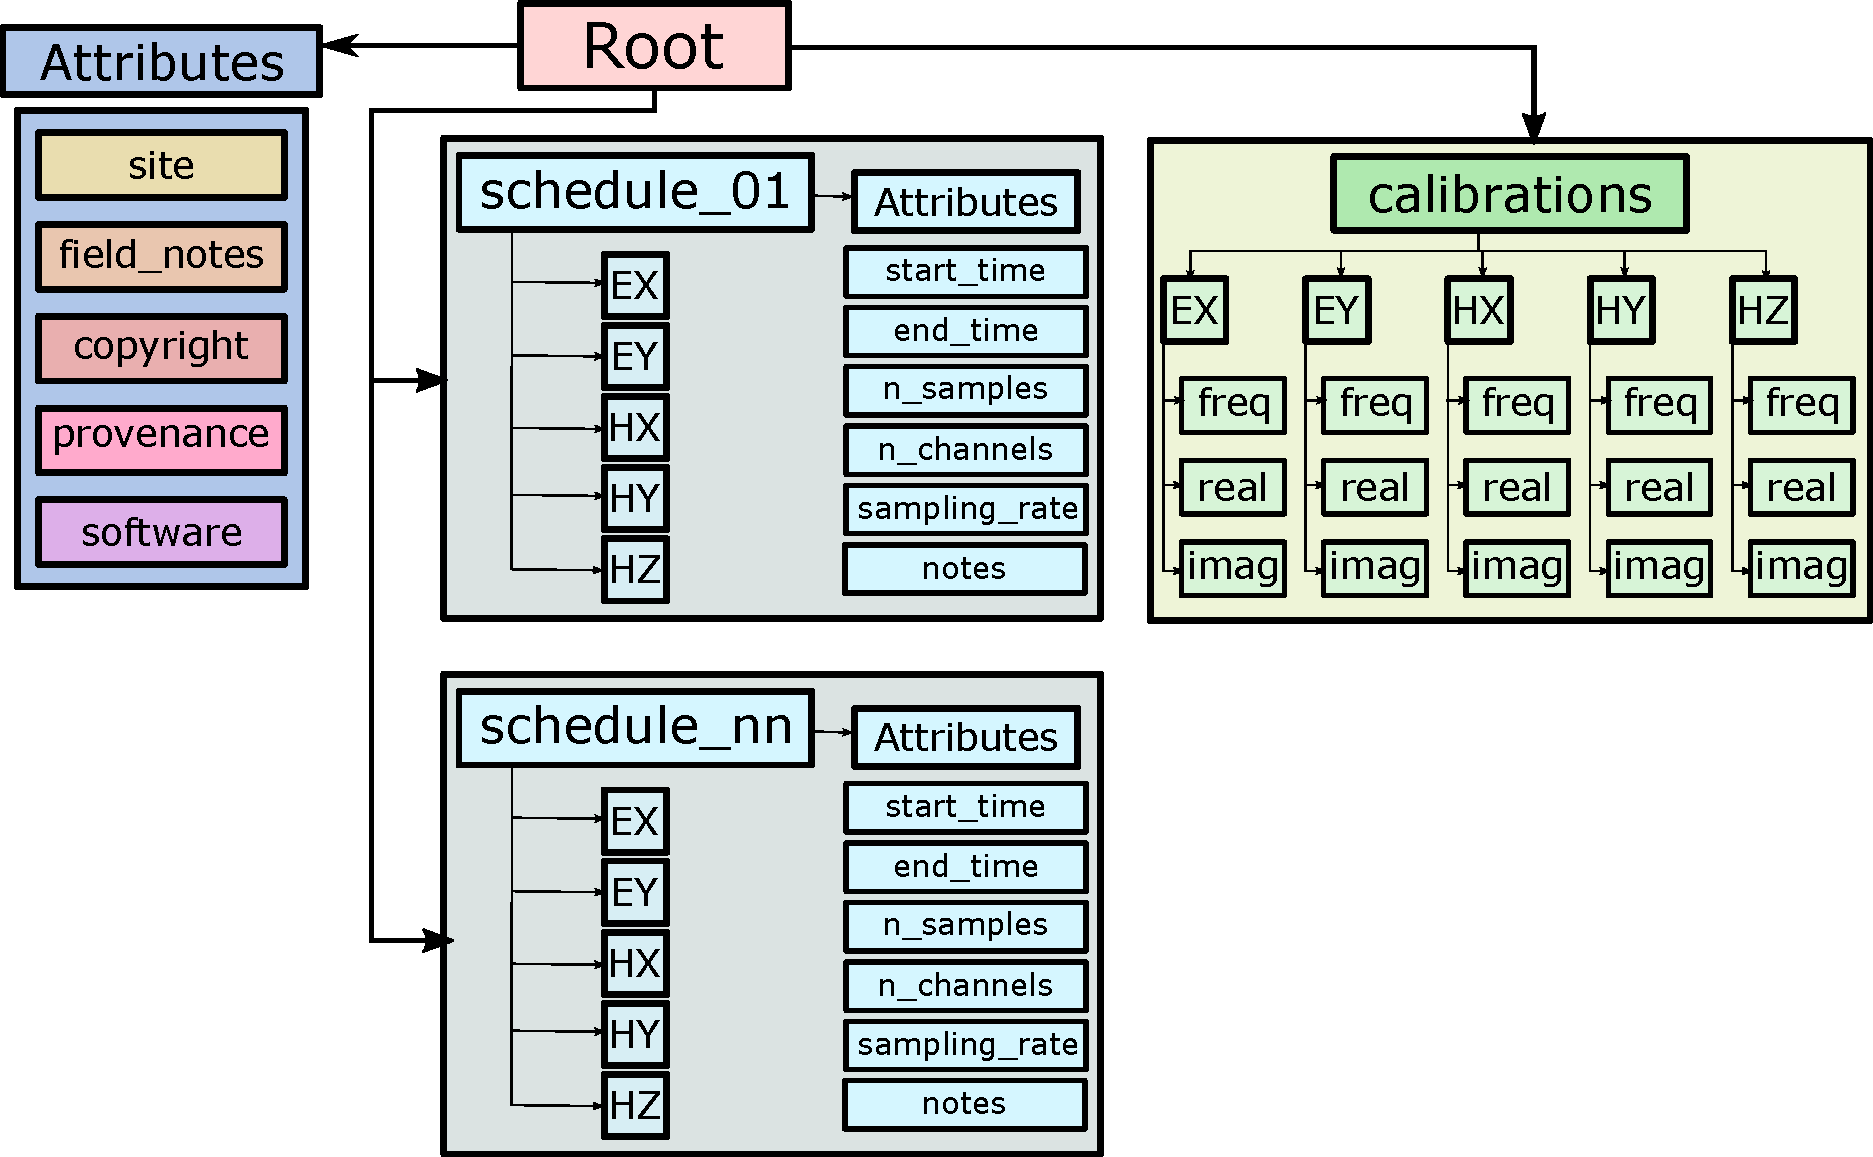
\includegraphics[width=.99\textwidth]{mth5_flowchart.pdf}
	\caption{Schematic of how an MTH5 file is setup.  See below for description of root attributes \attr{site}, \attr{field\_notes}, \attr{copyright}, \attr{provenance}, and \attr{software}.}
	\label{fig:flowchar}
\end{figure}

\subsection{Description of \textbf{site}}

\begin{itemize}
	\setlength{\itemsep}{.05em}
	\item \attr{acquired\_by, string}: who acquired the data
	\begin{itemize}
		\setlength{\itemsep}{.05em}
		\item \attr{email}: email of person responsible for the data
		\item \attr{name}: name of person responsible for the data
		\item \attr{organization}: organization name for person responsible for the data
		\item \attr{organization\_url}: organization website for person responsible for the data
	\end{itemize}
	\item \attr{coordinate\_system}: [ Geographic North $|$ Geomagnetic North $|$ something else ]
	\item \attr{datum}: Datum that represents the location coordinates, (WGS84)
	\item \attr{declination}: geomagnetic declination of station location
	\item \attr{declination\_epoch}: epoch from which declination is estimated
	\item \attr{elev\_units}: units of elevation [ meters $|$ feet $|$ something else ]
	\item \attr{elevation}: elevation of station in \attr{elev\_units}
	\item \attr{end\_date}: date and time of when recording stopped\footnote[1]{The preferred format is YYYY-MM-DDThh:mm:ss.ms UTC}.
	\item \attr{id}: name of the station
	\item \attr{latitude}: latitude of station\footnote[2]{Preferred format is decimal degrees}
	\item \attr{longitude}: longitude of station\footnotemark[2]
	\item \attr{start\_date}: date and time of when recording began\footnotemark[1]
	\item \attr{survey}: survey name and location  
\end{itemize}

\subsubsection{Example JSON encoded metadata for \textbf{site}}
\begin{verbatim}
	{"acquired_by": {"email": "generic@email.com",
	                 "name": "John Doe",
	                 "organization": "Company Name",
	                 "organization_url": "www.company_name.com"},
	"coordinate_system": "Geomagnetic North",
	"datum": "WGS84",
	"declination": 15.5,
	"declination_epoch": 1995,
	"elev_units": "meters",
	"elevation": 1111.72,
	"end_date": "2015-08-17T14:19:38.000000 UTC",
	"id": "mshH020",
	"latitude": 46.655559999999994,
	"longitude": -121.48472,
	"start_date": "2015-08-14T13:59:55.000000 UTC",
	"survey": "MT survey Washington, USA"}
\end{verbatim}

\newpage
\subsection{Description of \textbf{field\_notes}}
\begin{itemize}
	\setlength{\itemsep}{.05em}
	\item \attr{data\_logger}: information about the data logger
	\begin{itemize}
		\setlength{\itemsep}{.05em}
		\item \attr{id}: ID number of data logger
		\item \attr{manufacturer}: Name of manufacturer
		\item \attr{type}: type of data logger
	\end{itemize}
	\item \attr{data\_quality}: information about data quality
	\begin{itemize}
		\setlength{\itemsep}{.05em}
		\item \attr{author}: name of person assessing data quality
		\item \attr{comments}: comments on data quality
		\item \attr{rating}: [1--5] 1 -- poor, 5 -- great
		\item \attr{warnings\_comments}: comments on any warnings flagged
		\item \attr{warnings\_flags}: number of flags
	\end{itemize}
	\item \attr{electrode\_xx}: information for electric fields EX and EY
	\begin{itemize}
		\setlength{\itemsep}{.05em}
		\item \attr{azimuth}: heading of dipole relative to \attr{site.coordinate\_system}
		\item \attr{chn\_num}: channel number 
		\item \attr{contact\_resistance}: contact resistance in kOhms
		\item \attr{gain}: gain for electric channel
		\item \attr{id}: ID number of electrode(s)
		\item \attr{length}: dipole length in meters
		\item \attr{manufacturer}: electrode maker name
		\item \attr{type}: type of electrode
		\item \attr{units}: units of electric field data 
	\end{itemize}
	\item \attr{magnetoteter\_xx}: information for magnetic fields HX, HY, HZ
	\begin{itemize}
		\setlength{\itemsep}{.05em}
		\item \attr{azimuth}: heading of magnetotmeter relative to \attr{site.coordinate\_system}
		\item \attr{chn\_num}: channel number 
		\item \attr{gain}: gain for electric channel
		\item \attr{id}: ID number of electrode(s)
		\item \attr{manufacturer}: electrode maker name
		\item \attr{type}: type of electrode
		\item \attr{units}: units of electric field data 
	\end{itemize}
\end{itemize}

\newpage
\subsubsection{Example JSON encoded metadata for \textbf{field\_notes}}
\begin{verbatim}
{"data_logger": {"id": "ZEN18",
                 "manufacturer": "Zonge",
                 "type": "32-Bit 5-channel GPS synced"},
"data_quality": {"author": "C. Cagniard",
                 "comments": "testing",
                 "rating": 5,
                 "warnings_comments": "bad data at 2018-06-07T20:10:00.00",
                 "warnings_flag": 1},
"electrode_ex": {"azimuth": 15.5,
                 "chn_num": 4,
                 "contact_resistance": 1,
                 "gain": 1,
                 "id": 1,
                 "length": 100.0,
                 "manufacturer": "Borin",
                 "type": "Fat Cat Ag-AgCl",
                 "units": "mV"},
"electrode_ey": {"azimuth": 105.5,
                 "chn_num": 5,
                 "contact_resistance": 1,
                 "gain": 1,
                 "id": 2,
                 "length": 92.0,
                 "manufacturer": "Borin",
                 "type": "Fat Cat Ag-AgCl",
                 "units": "mV"},
"magnetometer_hx": {"azimuth": 15.5,
                    "chn_num": 1,
                    "gain": 1,
                    "id": 2374,
                    "manufacturer": "Geotell",
                    "type": "Ant 4 Induction Coil",
                    "units": "mV"},
"magnetometer_hy": {"azimuth": 105.5,
                    "chn_num": 2,
                    "gain": 1,
                    "id": 2384,
                    "manufacturer": "Geotell",
                    "type": "Ant 4 Induction Coil",
                    "units": "mV"},
"magnetometer_hz": {"azimuth": 90,
                    "chn_num": 3,
                    "gain": 1,
                    "id": 2514,
                    "manufacturer": "Geotell",
                    "type": "Ant 4 Induction Coil",
                    "units": "mV"}}
\end{verbatim}

\newpage
\subsection{Description of \textbf{copyright}} 

\begin{itemize}
	\setlength{\itemsep}{.05em}
	\item \attr{additional\_info}: any additional information about copyright
	\item \attr{citation}: Citation that uses this data
	\begin{itemize}
		\setlength{\itemsep}{.05em}
		\item \attr{author}: citation author
		\item \attr{doi}: doi number of citation
		\item \attr{journal}: name of publisher
		\item \attr{title}: citation title
		\item \attr{volume}: citation volume
		\item \attr{year}: citation year
	\end{itemize}
	\item \attr{conditions\_of\_use}: Conditions of using the data
	\item \attr{release\_status}: status of the data release
\end{itemize}

\subsubsection{Example JSON encoded metadata for \textbf{copyright}}
\begin{verbatim}
{"additional_info": "this is a test",
 "citation": {"author": "Tikhanov",
              "doi": "10.1023/usgs_mt_test",
              "journal": "SI",
              "title": "MT HDF5 test",
              "volume": 1,
              "year": 2018},
 "conditions_of_use": "All data and metadata for this survey are available free of charge 
                       and may be copied freely, duplicated and further distributed provided
                       this data set is cited as the reference. While the author(s) strive to
                       provide data and metadata of best possible quality, neither the author(s)
                       of this data set, not IRIS make any claims, promises, or guarantees about
                       the accuracy, completeness, or adequacy of this information, and expressly
                       disclaim liability for errors and omissions in the contents of this file.
                       Guidelines about the quality or limitations of the data and metadata, as 
                       obtained from the author(s), are included for informational purposes 
                       only.",
 "release_status": "Open to the public"} 
\end{verbatim}
   
\subsection{Description of \textbf{provenance}} 

\begin{itemize}
	\setlength{\itemsep}{.05em}
	\item \attr{creating\_application}: software used to create the file
	\item \attr{creation\_time}: creation date and time of file
	\item \attr{creator}: information about creator 
	\begin{itemize}
		\setlength{\itemsep}{.05em}
		\item \attr{email}: email of person who created file
		\item \attr{name}: name of person who created file
		\item \attr{organization}: organization of person who created file
		\item \attr{organization\_url}: organization URL of person who created file
	\end{itemize}
	\item \attr{submitter}: information about submitter 
	\begin{itemize}
		\setlength{\itemsep}{.05em}
		\item \attr{email}: email of person who submitted file
		\item \attr{name}: name of person who submitted file
		\item \attr{organization}: organization of person who submitted file
		\item \attr{organization\_url}: organization URL of person who submitted file
	\end{itemize}
\end{itemize}
   
\subsubsection{Example JSON encoded metadata for \textbf{provenance}}
\begin{verbatim}
{"creating_application": "MTH5py",
 "creation_time": "2017-11-27T21:54:49.00",
 "creator": {"email": "test@email.com",
             "name": "author",
             "organization": "company name",
             "organization_url": "https://www.company_name.com"},
 "submitter": {"email": "test@email.com",
               "name": "author",
               "organization": "company name",
               "organization_url": "https://www.company.com"}}
\end{verbatim}
  
\subsection{Description of \textbf{software}} 

\begin{itemize}
	\item \attr{author}: information about the author of the software used to make file
	\setlength{\itemsep}{.05em}
	\begin{itemize}
		\setlength{\itemsep}{.05em}
		\item \attr{email}: email of software author
		\item \attr{name}: name of software author
		\item \attr{organization}: organization of software author
		\item \attr{organization\_url}: organization URL software author
	\end{itemize}
	\item \attr{name}: software name that made file
	\item \attr{version}: software version 
\end{itemize}

\subsubsection{Example JSON encoded metadata for \textbf{provenance}}
\begin{verbatim}
{"author": {"email": "send@email.com",
            "name": "author",
            "organization": "company name",
            "organization_url": "https://company_name.com"},
 "name": "MTH5py",
 "version": "Beta"}
\end{verbatim}

\section{Calibrations}

Calibrations are put in a dedicated folder where each instrument calibration is put in a sub-folder.  Each instrument calibration folder can have metadata attributes.  These should contain information about units, date of calibration, and who did the calibration.  Typically the magnetometer calibrations are given as a complex value as a function of frequency or period.  These data are subsequently put in their own folder.

Attributes should include:
\begin{itemize}
	\setlength{\itemsep}{.1em}
	\item \attr{instrument\_id}: ID number of instrument 
	\item \attr{calibration\_date}: date of calibration\footnote[1]{The preferred format is YYYY-MM-DD}
	\item \attr{calibration\_person}:
	\begin{itemize}
		\setlength{\itemsep}{.05em}
		\item \attr{email}: email of person who did calibration
		\item \attr{name}: name of person who did calibration
		\item \attr{organization}: organization of person who did calibration
		\item \attr{organization\_url}: organization URL of person who did calibration
	\end{itemize} 
	\item \attr{units}: units of calibration
\end{itemize} 

\subsubsection{Example JSON encoded metadata for \textbf{calibration}}
\begin{verbatim}
{"calibration_date": "2010-10-01",
 "calibration_person": {"email": "test@email.com",
                        "name": "test",
                        "organization": "house",
                        "organization_url": "www.house.com"},
 "instrument_id": 2284,
 "name": "hx",
 "units": "mV/nT"}
\end{verbatim}

\section{Schedule Blocks}

Commonly MT measurements are recorded at different sampling rates over the course of a measurement to get the full range of data.  Or sometimes data recording may be interrupted and restarted.  The different recordings are labeled \verb|schedule_xx| where the \verb|xx| represents order of the measurement [0--n], labeled as a 2 character number, with a leading 0 if n is less than 10.  The first schedule is \verb|schedule_01| and the n$^{th}$ schedule is \verb|schedule_nn|. 

\textbf{Should the attributes be converted to JSON or left as is?}

The \verb|schedule_nn| folder has attributes attached to it.  These are:

\begin{itemize}
	\setlength{\itemsep}{.1em}
	\item \attr{start\_time}: date and time data recording started\footnote[1]{The preferred format is YYYY-MM-DDThh:mm:ss.ms UTC}
	\item \attr{end\_time}: date and time data recording ended\footnotemark[1]
	\item \attr{start\_seconds}: seconds from the epoch (1970-01-01) data recording started
	\item \attr{end\_seconds}: seconds from the epoch (1970-01-01) data recording ended
	\item \attr{sampling\_rate}: sampling rate in samples/second
	\item \attr{n\_samples}: number of samples in each channel
	\item \attr{n\_channels}: number of channels recorded
\end{itemize}  

   

\end{document}
